\documentclass[xcolor={dvipsnames}]{beamer}

\usepackage{algorithm2e}
\usepackage{multicol}
\usepackage{tikz}
\usetikzlibrary{fit}
\pgfdeclarelayer{background}
\pgfsetlayers{background,main}

\setbeamertemplate{navigation symbols}{}

%% Borrowed from the Altran LaTeX style
\usepackage{listings}
\lstdefinelanguage{SPARK}{
  language = [95]Ada,
  morekeywords = {pre,post,assert,assume,check,derives,hide,global,depends,inherit,from,own,initializes,main_program,assert,loop_variant,loop_invariant,increases,decreases,ghost,spark_mode,abstract_state,refined_state,refined_global,refined_depends},
  comment=[l][commentstyle]{--\ },
  texcl=true,
  showstringspaces=false
}
\lstdefinestyle{tinystyle}
   {basicstyle=\scriptsize\tt,
    keywordstyle=\color{RoyalBlue},
    commentstyle=\rmfamily\it\color{Sepia},
    captionpos=b,
    caption={},label={},
    numbers=none,
    escapeinside={(*}{*)}}
\lstset{language=SPARK}
\lstset{style=tinystyle}



\title{Generated Globals With Partitions}
\author{Florian Schanda}

\begin{document}

\maketitle

\begin{frame}{The problem}
  Transitioning from one level of abstraction to another cannot be resolved
  currently and leads to difficult to understand misbehaviour.

  \begin{center}
    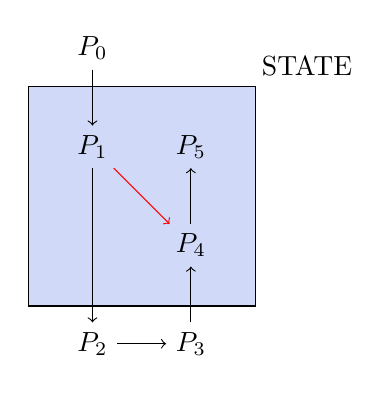
\begin{tikzpicture}[x=1.25cm,y=-1.25cm]

      \node (p0) at (0, 0) {$P_0$};
      \node (p1) at (0, 1) {$P_1$};
      \node (p2) at (0, 3) {$P_2$};
      \node (p3) at (1, 3) {$P_3$};
      \node (p4) at (1, 2) {$P_4$};
      \node (p5) at (1, 1) {$P_5$};

      \begin{pgfonlayer}{background}
        \node (q) [
          draw,
          inner sep=0.5cm,
          fill=RoyalBlue!25,
          fit=(p1) (p4) (p5),
          label=above right:STATE
        ] {};
      \end{pgfonlayer}

      \draw[->] (p0) -- (p1);
      \draw[->] (p1) -- (p2);
      \draw[->] (p2) -- (p3);
      \draw[->] (p3) -- (p4);
      \draw[->] (p4) -- (p5);

      \draw<2->[red,->] (p1) -- (p4);
    \end{tikzpicture}
  \end{center}

  \begin{itemize}
  \item<2->In particular: $P_1$ must not use the refined globals of $P_4$!
  \end{itemize}
\end{frame}

\begin{frame}{Phase 1}{Overall approach}
  \begin{itemize}
  \item Recursive descent, instead of arbitrary order of analysis
  \item Close graphs and project as we move up (abstraction)
    \begin{itemize}
    \item Effects from calls down ``\structure{local}'' are made using the
      closed graph created so far
    \item Effects from calls up ``\structure{remote}'' are resolved once we
      close the graph for that scope
    \end{itemize}
  \item Summarize state for un-annotated packages (abstraction)
  \item Save original graphs before projection (refined globals)
  \item Strip local variables as we move up (efficiency)
  \item Less complex graphs with fewer vertices (efficiency)
  \item Integrates perfectly with annotations (sanity)
  \end{itemize}
\end{frame}

\begin{frame}{Phase 1}{The global graph}
  A global graph contains the following basic elements:
  \begin{itemize}
  \item Variables, abstract state
  \item Names of procedures
  \end{itemize}

  And for each subprogram (and package elaboration) we have nodes that link
  to the above or each other:
  \begin{itemize}
  \item Locally declared variables (or parameters)
  \item Variables read
  \item Variables wrote (mode out)
  \item Remote subprograms called
  \item Remote subprograms possibly called
  \end{itemize}
\end{frame}

\begin{frame}{Phase 1}{Local calls}
  A \structure{local} call is on the same level of scope, or to an
  arbitrarily nested scope. A call from $P_1$ to $P_2$ generates the
  following links in the graph:
  \begin{itemize}
  \item $reads(P_1) \rightarrow reads(P_2)$
  \item $writes(P_1) \rightarrow writes(P_2)$
  \item $calls(P_1) \rightarrow calls(P_2)$
  \item $maybe(P_1) \rightarrow maybe(P_2)$
  \end{itemize}

  A \structure{local} maybe call from $P_1$ to $P_2$ generates the
  following links in the graph:
  \begin{itemize}
  \item $reads(P_1) \rightarrow \{reads(P_2), writes(P_2)\}$
  \item $writes(P_1) \rightarrow writes(P_2)$
  \item $maybe(P_1) \rightarrow \{calls(P_2), maybe(P_2)\}$
  \end{itemize}
\end{frame}

\begin{frame}{Phase 1}{Remote calls}
  A \structure{remote} call is anything a local call is not; i.e. to a
  different package or a call to an enclosing scope. A call from $P$ to $R$
  generates the following links in the graph:
  \begin{itemize}
  \item $calls(P) \rightarrow R$
  \end{itemize}

  A \structure{remote} maybe call from $P$ to $R$ generates the following
  links in the graph:
  \begin{itemize}
  \item $maybe(P) \rightarrow R$
  \end{itemize}
\end{frame}

\begin{frame}[fragile]{Example}
  \begin{multicols}{2}
    \begin{lstlisting}[gobble=6]
      package body Outer
         package body Inner
            X : Boolean;
            Y : Boolean;
            Z : Boolean;

            procedure P0 is begin
               X := False;
               P1;
            end P0;

            procedure P2 is begin
               Y := False;
               P3;
            end P2;

            procedure P3 is begin
               Z := False;
            end P3;
         end Inner;
    \end{lstlisting}
    \vfill\columnbreak
    \begin{lstlisting}[gobble=6]
         procedure P1 is begin
            Inner.P2;
         end P1;
      end Outer;
    \end{lstlisting}
  \end{multicols}
\end{frame}

\begin{frame}{Example}
  \begin{center}
    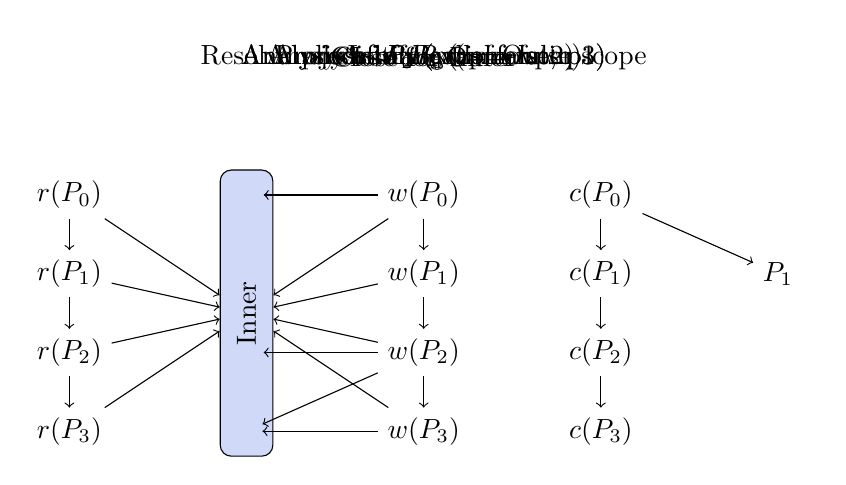
\begin{tikzpicture}[x=2.25cm,y=-1cm]
      \tikzstyle{lbl}=[minimum width=10cm,minimum height=0.75cm,align=left]
      \coordinate(lp) at (2.0,-1.75);
      \node<1> [lbl] at (lp) {Initial graph};
      \node<2> [lbl] at (lp) {Analysis of $P_0$ (x := false; p1)};
      \node<3> [lbl] at (lp) {Analysis of $P_2$ (y := false; p3)};
      \node<4> [lbl] at (lp) {Analysis of $P_3$ (z := false)};
      \node<5> [lbl] at (lp) {Close for Inner};
      \node<6> [lbl] at (lp) {Project to view of Outer};
      \node<7> [lbl] at (lp) {Resolve procedure calls now in scope};
      \node<8> [lbl] at (lp) {Analysis of $P_1$ (inner.p2)};
      \node<9> [lbl] at (lp) {Close for Outer};

      \node<1-5> (x)  at (1, 0) {x};
      \node      (p1) at (4, 1) {$P_1$};
      \node<1-5> (y)  at (1, 2) {y};
      \node<1-5> (z)  at (1, 3) {z};
      \node<6->  (inner) [draw,fill=RoyalBlue!25,
                          fit=(x) (y) (z),
                          rounded corners] {};
      \node<6-> [rotate=90] at (inner) {Inner};

      \node (p0_read) at (0, 0) {$r(P_0)$};
      \node<6-> (p1_read) at (0, 1) {$r(P_1)$};
      \node (p2_read) at (0, 2) {$r(P_2)$};
      \node (p3_read) at (0, 3) {$r(P_3)$};

      \node (p0_write) at (2, 0) {$w(P_0)$};
      \node<6-> (p1_write) at (2, 1) {$w(P_1)$};
      \node (p2_write) at (2, 2) {$w(P_2)$};
      \node (p3_write) at (2, 3) {$w(P_3)$};

      \node (p0_call) at (3, 0) {$c(P_0)$};
      \node<6-> (p1_call) at (3, 1) {$c(P_1)$};
      \node (p2_call) at (3, 2) {$c(P_2)$};
      \node (p3_call) at (3, 3) {$c(P_3)$};

      \draw<2-5>[->] (p0_write) -- (x);
      \draw<2-6>[->] (p0_call) -- (p1);

      \draw<3-5>[->] (p2_write) -- (y);
      \draw<3-5>[->] (p2_read)  -- (p3_read);
      \draw<3-5>[->] (p2_write) -- (p3_write);
      \draw<3->[->] (p2_call)  -- (p3_call);

      \draw<4-5>[->] (p3_write) -- (z);

      \draw<5>[->] (p2_write) -- (z);

      \draw<6->[->] (p0_write) -- (inner);
      \draw<6->[->] (p2_write) -- (inner);
      \draw<6->[->] (p3_write) -- (inner);
      \draw<6->[->] (p0_read) -- (inner);
      \draw<6->[->] (p2_read) -- (inner);
      \draw<6->[->] (p3_read) -- (inner);

      \draw<7->[->] (p0_read)  -- (p1_read);
      \draw<7->[->] (p0_write) -- (p1_write);
      \draw<7->[->] (p0_call)  -- (p1_call);

      \draw<8->[->] (p1_read)  -- (p2_read);
      \draw<8->[->] (p1_write) -- (p2_write);
      \draw<8->[->] (p1_call)  -- (p2_call);

      \draw<9->[->] (p1_read)  -- (inner);
      \draw<9->[->] (p1_write) -- (inner);

    \end{tikzpicture}
  \end{center}
\end{frame}


\end{document}
